\documentclass[a4paper,12pt]{article}
%spellchecker
% !TeX spellcheck = de

\usepackage{amssymb} % needed for math
\usepackage{amsmath} % needed for math
\usepackage[utf8]{inputenc} % this is needed for german umlauts
\usepackage[ngerman]{babel} % this is needed for german umlauts
\usepackage[T1]{fontenc}    % this is needed for correct output of umlauts in pdf
\usepackage[margin=2.5cm]{geometry} %layout
\usepackage{booktabs}



% this is needed for forms and links within the text
\usepackage{hyperref}  

% Generate the glossary
\usepackage[nonumberlist]{glossaries}
\makeglossary

% The following is needed in order to make the code compatible
% with both latex/dvips and pdflatex.
\ifx\pdftexversion\undefined
\usepackage[dvips]{graphicx}
\else
\usepackage[pdftex]{graphicx}
\DeclareGraphicsRule{*}{mps}{*}{}
\fi

%%%%%%%%%%%%%%%%%%%%%%%%%%%%%%%%%%%%%%%%%%%%%%%%%%%%%%%%%%%%%%%%%%%%%%
% Variablen                                 						 %
%%%%%%%%%%%%%%%%%%%%%%%%%%%%%%%%%%%%%%%%%%%%%%%%%%%%%%%%%%%%%%%%%%%%%%
\newcommand{\authorName}{Lena Gregor, Dominik Horn}
\newcommand{\auftraggeber}{Lehrstuhl für Datenbanksysteme TUM}
\newcommand{\auftragnehmer}{\authorName}
\newcommand{\projektName}{Wahl und Informationssystem für bayerische Landtagswahlen}
\newcommand{\tags}{\authorName, Pflichtenheft, TUM, Universität Augsburg, LMU}
\newcommand{\subtitle}{Technische Universität München, Datenbanksysteme WS19/20}
\newcommand{\glossarName}{Glossar}

%%%%%%%%%%%%%%%%%%%%%%%%%%%%%%%%%%%%%%%%%%%%%%%%%%%%%%%%%%%%%%%%%%%%%%
% PDF Meta information                                 				       %
%%%%%%%%%%%%%%%%%%%%%%%%%%%%%%%%%%%%%%%%%%%%%%%%%%%%%%%%%%%%%%%%%%%%%%
\hypersetup{
  pdfauthor   = {\authorName},
  pdfkeywords = {\tags},
  pdftitle    = {\projektName~(Pflichtenheft)}
} 

%%%%%%%%%%%%%%%%%%%%%%%%%%%%%%%%%%%%%%%%%%%%%%%%%%%%%%%%%%%%%%%%%%%%%%
% Custom setup                                                       % 
%%%%%%%%%%%%%%%%%%%%%%%%%%%%%%%%%%%%%%%%%%%%%%%%%%%%%%%%%%%%%%%%%%%%%%
\usepackage{pdfpages}
\usepackage{xcolor,colortbl} 
\definecolor{Blue}{rgb}{0.1,0.2,0.7}
\definecolor{TUMBlue}{HTML}{0065BD}
\definecolor{TUMSecondaryBlue}{HTML}{005293}
\definecolor{TUMSecondaryBlue2}{HTML}{003359}
\definecolor{TUMAccentBlue}{HTML}{64A0C8}
\definecolor{TUMAccentLightBlue}{HTML}{98C6EA}
\definecolor{lightBlue}{RGB}{157,195,230}


\newcolumntype{a}{>{\columncolor{TUMBlue}}c}
\newcolumntype{b}{>{\columncolor{lightBlue}}c}

\renewcommand{\arraystretch}{1.5}
 
%%%%%%%%%%%%%%%%%%%%%%%%%%%%%%%%%%%%%%%%%%%%%%%%%%%%%%%%%%%%%%%%%%%%%%
% Create a shorter version for tables. DO NOT CHANGE               	 %
%%%%%%%%%%%%%%%%%%%%%%%%%%%%%%%%%%%%%%%%%%%%%%%%%%%%%%%%%%%%%%%%%%%%%%
\newcommand\addrow[2]{\textcolor{black}{#1} &#2\\ \hline}

\newcommand\addheading[2]{\rowcolor{TUMBlue}\textcolor{white}{#1} & \textcolor{white}{#2}\\ \hline}
\newcommand\tabularhead{\begin{tabular}{|b|p{13cm}|}
\hline
}

\newcommand\addmulrow[2]{ \begin{minipage}[t][][t]{2.5cm}#1\end{minipage}% 
   &\begin{minipage}[t][][t]{8cm}
    \begin{enumerate} #2   \end{enumerate}
    \end{minipage}\\ }

\newenvironment{usecase}{\tabularhead}
{\hline\end{tabular}}

%%%%%%%%%%%%%%%%%%%%%%%%%%%%%%%%%%%%%%%%%%%%%%%%%%%%%%%%%%%%%%%%%%%%%%
% THE DOCUMENT BEGINS             	                              	 %
%%%%%%%%%%%%%%%%%%%%%%%%%%%%%%%%%%%%%%%%%%%%%%%%%%%%%%%%%%%%%%%%%%%%%%
\begin{document}
 \pagenumbering{roman}
 \begin{titlepage}
\maketitle
\thispagestyle{empty} % no page number

\begin{verbatim}












\end{verbatim}


  \begin{tabular}[t]{ll}
	Projekt:       & \quad \projektName \\[1.2ex]
	Auftraggeber:  & \quad \auftraggeber\\[1.2ex]
	Auftragnehmer: & \quad \auftragnehmer\\[1.2ex]
  \end{tabular}

\begin{tabular}{|p{3 cm}|p{3 cm}|p{5 cm}|}
\hline
\textbf{Version} & \textbf{Datum} & \textbf{Autor(en)} \\
\hline
\hline
1.0 & 04.11.2019 & \authorName \\
\hline
\end{tabular}
\end{titlepage}
         % Deckblatt.tex laden und einfügen
 \setcounter{page}{2}

 \tableofcontents          % Inhaltsverzeichnis ausgeben
 \clearpage
 \pagenumbering{arabic}
 
\section{Zielbestimmung}
%%%%%%%%%%%%%%%%%%%%%%%%%%%%%%%%%%%%%%%%%%%%%%%%%%%%%%%%%%%%%%%%%%%%%%
% Warum wird das Projekt gemacht?           						 %
%%%%%%%%%%%%%%%%%%%%%%%%%%%%%%%%%%%%%%%%%%%%%%%%%%%%%%%%%%%%%%%%%%%%%%
Der Freistaat Bayern möchte in Kooperation mit dem Lehrstuhl für 
Datenbanksysteme an der Technischen Universität München eine digitales 
Wahlinformations- und Stimmabgabesystem für Landtagswahlen mithilfe von 
Studierenden des Elite Software Engineering Masterstudiengangs aufbauen.
%
Das System soll dabei nicht nur die Ergebnisse für die Landtagswahlen 
2013 und 2018, wie z. B. die Sitzverteilung im Landtag, die statistische Auswertung von Ergebnissen oder die Berechnung gewonnener
Mandate, analysier- und vergleichbar machen, sondern auch als sicheres System für die elektronische 
Stimmabgabe im Wahllokal dienen. 
%
Es müssen die gesetzlichen Regelungen, Normen und Datenschutzaspekte
berücksichtigt werden. Als Basis gelten die Regelungen zur
Landtagswahl 2018


\subsection{Musskriterien}
% Requirements
\begin{usecase}
	\addheading{Nummer}{Die Anwendung ermöglicht es...} 
      \addrow{M01}{...WählerInnen Einzelstimmen abzugeben nach vorangestellter Freigabe durch eine(n) WahlhelferIn.}
      \addrow{M02}{...im Echtbetrieb, dass mehrere Stimmen gleichzeitig abgegeben werden können.}
      \addrow{M03}{...selbst im Katastrophenfall persistierte Wahldaten zu recovern.}
	\addrow{M04}{...Daten von vergangenen Wahlen mit Hilfe einer CSV-Datei fehlerfrei in das System einzuspeisen und statistisch auszuwerten.}
	\addrow{M05}{...bei der statistischen Auswertung die Verteilung der Sitze, die Auswertung für die Direkt- und Listenmandate und die Anzahl der Stimmen pro Partei einzusehen.}
	\addrow{M06}{...pro Stimmkreis die Einzelstimmen zu Stimmkreisergebnissen vorzuaggregieren.}
	\addrow{M07}{...erst nach Abschluss einer Wahl diese statistisch auszuwerten, um z. B. die Wahlbeeinflussung oder timed-attacks auf das Wahlgeheimnis zu verhindern.}
      \addrow{M08}{Das System beachtet alle relevanten gesetzlichen Vorgaben für die bayerische Landtagswahlen, wie z. B. die getrennte Speicherung von Erst- und Zweitstimmen, um das Wahlgeheimnis und weitere Datenschutzaspekte zu respektieren und zu erfüllen.}
\end{usecase}

\subsection{Sollkriterien}
\begin{usecase}
	\addheading{Nummer}{Beschreibung} 
	\addrow{S01}{Die Anwendung ermöglicht es dem Anwender die Ergebnisse von unterschiedlichen Wahlen in einer Ansicht zu vergleichen.}
      \addrow{S02}{Die Oberfläche zur statistischen Auswertung ist frei zugänglich, die zur Stimmabgabe (durch Wähler oder Wahlhelfer/ -leiter) je nur für Berechtigte.}
      \addrow{S03}{Das System ist hinreichend gegen unbefugte Zugriffe abgesichert, sodass es akzeptabel wäre im Realbetrieb}
\end{usecase}
\subsection{Kannkriterien}
\begin{usecase}
	\addheading{Nummer}{Beschreibung} 
	\addrow{K01}{Die Anwendung kann bei der statistischen Auswertung Ergebnisse auf einer Landkarte visualisieren.}
      \addrow{K02}{Es ist möglich gültige oder ungültige Stimmen abzugeben und in das System einzutragen.}
\end{usecase}

\subsection{Abgrenzungskriterien}
\begin{usecase}
      \addheading{Nummer}{Das System...} 
      \addrow{A01}{...ist keine volle E-Voting Plattform, sondern ist lediglich imstande Stimmen von WählerInnen in Wahlkabinen entgegen zu nehmen.}
	\addrow{A02}{...kann nicht die Berechtigung von WählerInnen überprüfen, sondern überlässt dies, wie aktuell praktiziert, den WahlhelferInnen.}
	\addrow{A03}{...verarbeitet und berechnet keine juristischen Ausnahmefälle, die bei den Wahlen 2013 und 2018 nicht relevant waren.}
\end{usecase}

\section{Technische Umsetzung}
Dieser Abschnitt widmet sich der geplanten technischen Realisierung
des Systems. Zunächst werden dazu anhand der Einsatzszenarien die Implementierungsidee
grob vorgestellt. Im darauf folgenden Abschnitt findet sich eine tabellarische 
Auflistung aller eingesetzten Technologien. Abschließend
wird der jeweilige Implementierungsansatz für alle Musskriterien beschrieben.

\subsection{Produkteinsatz und Umgebung}
Die Anwendung ist konzipiert und entwickelt um die Stimmabgabe 
zu bayerischen Landtagswahlen (Erst-, Zweitstimme) durch wahlberechtigte
Personen, sowie die (statistische) Auswertung von Wahlergebnissen zu ermöglichen. 
%
Das System wird in verschiedenen Gebieten eingesetzt:

\begin{center}
\begin{tabular}{|m{5cm}|m{10cm}|}
	\hline
  \rowcolor{TUMBlue} \textcolor{white}{\textbf{Einsatzgebiet}} & \textcolor{white}{\textbf{Prozesse}} \\
  \hline
  Wahllokal & Abgabe von Einzelstimmen durch WählerInnen und batch Stimmeintragung durch WahlhelferInnen \\
	\hline
  Bürgerlicher Gebrauch & (statistische-)Analyse von Wahlergebnissen \\
  \hline
  Staatlicher Gebrauch & (statistische-)Analyse von Wahlergebnissen, Import von alten Wahlergebnissen \\
	\hline
\end{tabular}
\end{center}

Die (statistische) Analyse und Auswertung von Wahlergebnissen erfolgt in einer frei zugänglichen
Weboberfläche, welche auf ein Backendsystem zur Datenbeschaffung zugreift. 
Während eines Wahlvorgangs sind Daten zum aktuellen Vorgang nicht (statistisch-) auswertbar, um unter anderem eine Beeinflussung oder Verfälschung des Wahlausgangs zu vermeiden.
Ebenso stellt das System sicher, dass keine Rückschlüsse auf Einzelne durch das Auswertungstool
möglich sind.

Das Interface zur Stimmabgabe sowie die von WahlhelferInnen und WahlleiterInnen zu benutzenden Oberflächen sind 
ebenfalls mit Webtechnologien implementiert, jedoch zugriffsbeschränkt und nicht über das Internet aufrufbar. Sie greifen
auf das selbe Backendsystem wie die Oberfläche zur (statistischen) Analyse zu.

Der durchgängige Einsatz von Webtechnologien senkt unter anderem den Projektaufwand, da die Entwickler sich für das gesamte System nur in 
einem einzigen Technologiestack bewegen müssen. Weiterhin sind insbesondere 
Webtechnologien dafür geeignet Geräte- und Bildschirmgrößen-unabhängige Software zu erstellen. Dies trägt dazu bei, dass eine Festlegung auf ein bestimmtes Gerät für die Stimmabgabe oder für die statistische Auswertung, zur Entwicklungszeit noch nicht notwendig ist. 

Die Implementierung des Backendsystems erfolgt als minimale Softwareschicht auf einem externen 
Rechner, fortan \textit{server} genannt. Jede Benutzeroberfläche schickt Anfragen, egal ob lesend oder schreibend, 
an den Server. Dieser führt die jeweilige Operation aus und liefert gegebenenfalls hervorgebrachte
Anfrageergebnisse wieder zurück an den Rechner auf welchem die Benutzeroberfläche angezeigt wird, fortan \textit{client}.

Jede Personengruppe kann zu jeder Zeit immer nur auf die für sie relevanten Interfaces zugreifen.
Dies steigert primär die Intuitivität der Benutzeroberfläche und minimiert potentielle Verwirrung
bei Benutzern. Die Absicherung des Systems beruht hingegen explizit nicht auf den getrennten 
Oberflächen. Vielmehr wird das Backendsystem durch Nutzerauthentifizierung der WahlleiterInnen und 
WahlhelferInnen, sowie Authentifizierung der einzelnen Wahllokale gesichert. Hierzu erhält der oder die 
WahlleiterIn sowie jede(r) WahlhelferIn vor jeder Landtagswahl einen sich je unterscheidenden 
Zugriffscode auf einem staatlich gesicherten, externen Kommunikationskanal. Dieser
ist jeweils nur für die Aufgabenbeschreibung der jeweiligen Person an dem für sie vorgesehenen Arbeitsplatz einsetzbar. Jeder Wahlkabine wird überdies je ein eindeutig identifizierbarer und von WahlhelferInnen autorisierter Zugriffscode
zugeordnet. Die Stimmabgabe ist nur mit einem autorisierten Wahlkabinen-Zugriffscode möglich und auch
nur dann, wenn ein(e) WahlhelferIn die Wahlkabine freigegeben hat. Die Freigabe einer Wahlkabine
ist immer nur für genau eine Stimmabgabe gültig.

Zur Persistierung von Daten durch das Backendsystem wird ein zugriffsgesichertes Datenbanksystem eingesetzt. Dieses
wird exklusiv von der durch das Projektteam implementierten Softwareschicht auf dem Server angesprochen.
Das bedeutet, dass die Backendsoftware lediglich als Proxy zwischen BenutzerIn und Datenbanksystem agiert. Sämtliche 
kritischen Datenzugriffe erfolgen stets authentifiziert.
%
Der Einsatz eines DBMS wird durch mehrere inhärente Vorteile begünstigt:

\begin{itemize}
      \item Parallele OLAP Abfragen sind ohne Zusatzaufwand möglich. So können z. B. mehrere BenutzerInnen gleichzeitig ungehindert voneinander die Wahlergebnisse statistisch auswerten.
      \item Mehrbenutzer OLTP out-of-the-box, z. B. können mehrere WählerInnen und WahlhelferInnen parallel Stimmen
            eintragen.
      \item Hohe Ausfallsicherheit, wie z. B., das System läuft stabil über längere Zeiträume.
      \item Recovery Funktionalität: falls z. B. ein Unglück geschieht (Brand im Datencenter, Stromausfall) 
            oder der Server abstürzt gehen keine Daten verloren, solange die entsprechenden DBMS features 
            (logging, backup) genutzt werden.
      \item Die Datenzugriffsschnittstelle ist standardisiert und flexibel (SQL).
      \item Integritätsbedingungen werden über das Datenbankschema automatisch realisiert
\end{itemize}

\subsection{Eingesetzte Technologien}
Der vorherige Abschnitt identifiziert zur Umsetzung des Systems folgende Softwarekomponenten:
\begin{itemize}
      \item Datenbanksystem zur Persistierung von Anwendungsdaten, d.h., Wahldaten zur bayerischen Landtagswahl
      \item Server Software zur Annahme und Bearbeitung von Client-Anfragen, insbesondere auch zur Ansteuerung des Datenbanksystems
      \item Client Software, je eine für die Stimmabgabe, für Wahlhelfer, Wahlleiter und zur (statistischen-) Auswertung von Wahlergebnissen 
\end{itemize}
Im folgenden werden die Haupttechnologien zur Umsetzung dieser Systemkomponenten tabellarisch aufgelistet. Abbildung \ref{fig:architecture} zeigt
deren Interaktion und Aufbau graphisch.

\begin{center}
      \begin{tabular}{|m{4cm}|m{2.5cm}|m{8.5cm}|}
            \hline
        \rowcolor{TUMBlue} \textcolor{white}{\textbf{Funktion/Gebiet}} & \textcolor{white}{\textbf{Eingesetzte Technologie}} & \textcolor{white}{\textbf{Erläuterung}} \\
        \hline
        Programmiersprache & TypeScript & TypeScript ist eine von Microsoft entwickelte Programmiersprache, welche JavaScript hauptsächlich um statische Typisierungsfähigkeiten ergänzt. Sie ist die Implementierungssprache für alle Softwarebereiche dieses Projekt.s \\
        \hline
        Datenbanksystem & PostgreSQL & PostgreSQL ist ein von der Industrie großflächig eingesetztes kostenfreies DBMS mit sehr guter Reputation und erprobtem Produktiveinsatz in großen Anwendungen. \\
        \hline
        Server & NodeJS & NodeJS ermöglicht es plattformunabhängig JavaScript Code auszuführen. Hier dient es dazu, die Serversoftware auszuführen. \\
        \hline
        Serverschnittstelle & Apollo Server & Apollo Server implementiert die notwendige serverseitige Funktionalität um auf GraphQL Anfragen zu antworten. Jeder request wird auf eine resolver-Funktion gemapped, welche sich darum kümmert die angeforderte Funktion (Daten lesen, Daten schreiben) auszuführen. \\
        \hline
        Anfragen senden & Apollo Client & Apollo Client implementiert die notwendige, clientseitige Funktionalität um GraphQL-Anfragen an einen Server zu schicken und die jeweiligen Antworten zu empfangen. \\
        \hline
        Frontend Basis & React & React ist ein von Facebook entwickeltes UI-Framework und wird zur Darstellung sämtlicher Inhalte verwendet. \\
        \hline
        Frontend UI & Ant Design & Ant Design ist eine React Component Library, welche viele nützliche GUI-Elemente vorgefertigt bereitstellt. \\
        \hline
      \end{tabular}
\end{center}

\begin{figure}[h!]
      \centering
      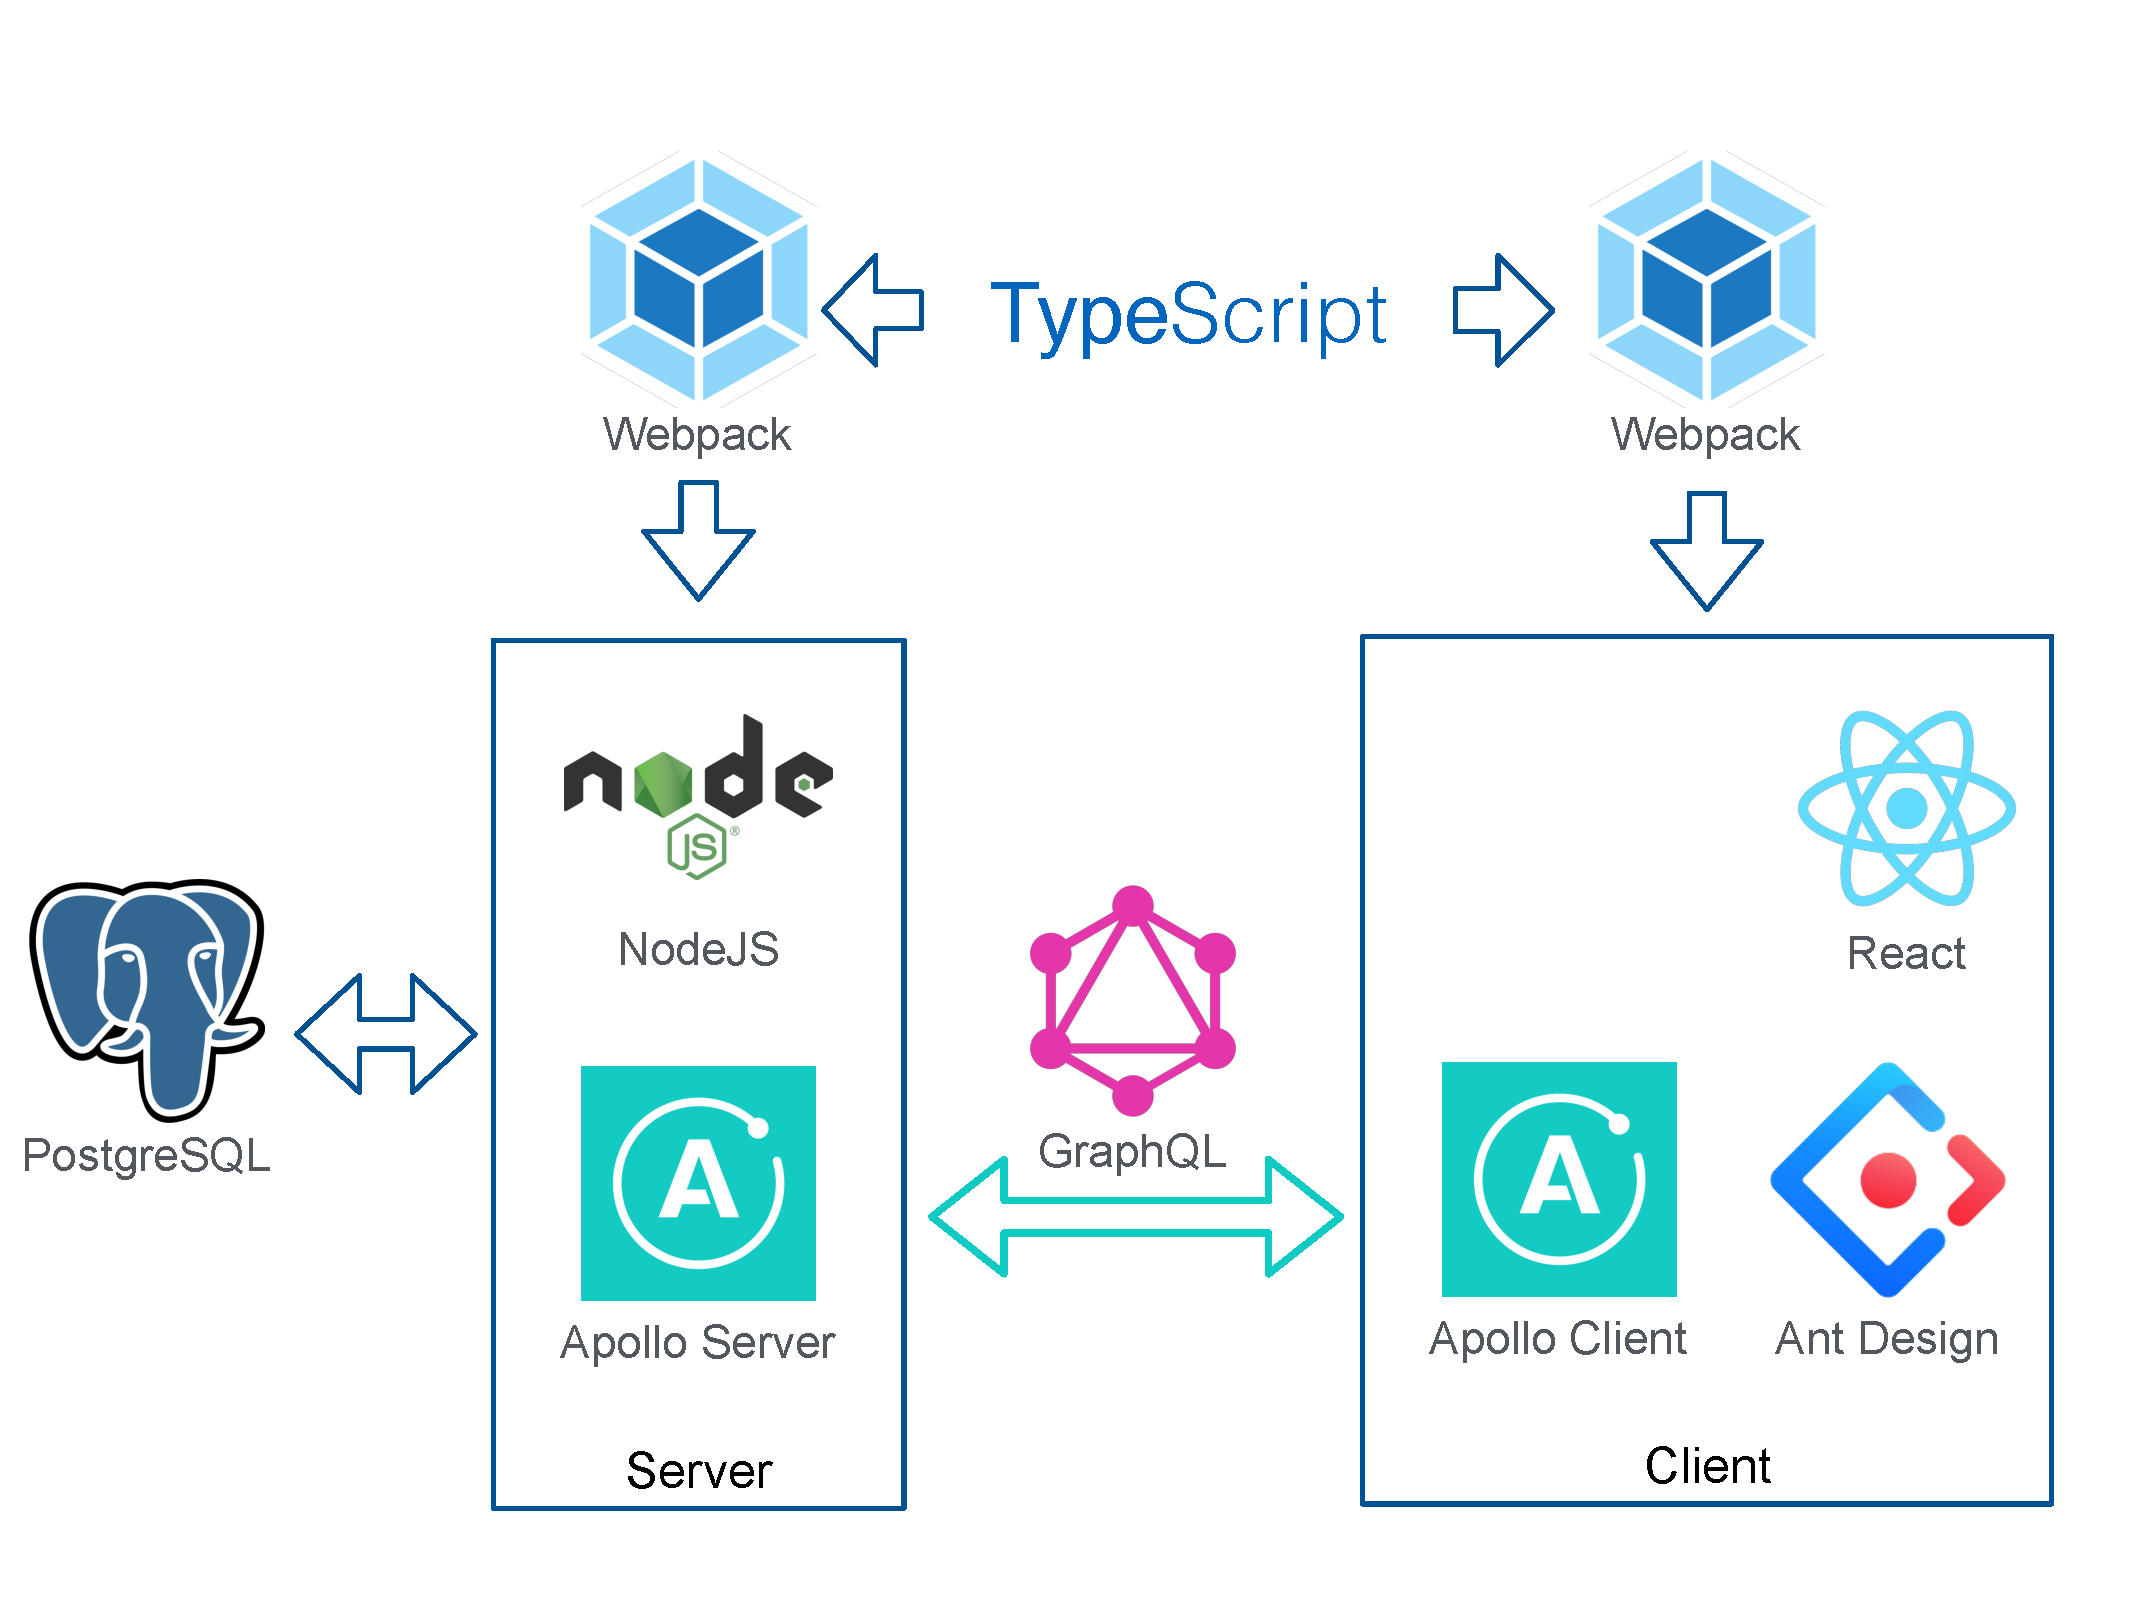
\includegraphics[width=\textwidth]{architecture.pdf}
      \caption{Illustrierung der Architektur und Interaktion von Systemkomponenten}
      \label{fig:architecture}
\end{figure}

\clearpage

\subsection{Erreichen der Zielsetzung}
Die definierten Kriterien und Systemeigenschaften werden durch die eingesetzten Technologien 
offensichtlich erreicht, sofern dieser Abschnitt sie nicht gesondert nennt.

\begin{usecase}
	\addheading{Nummer}{Zielsetzung wird erreicht, weil:} 
      \addrow{M01}{Der oder die WahlhelferIn in einer separaten Oberfläche die individuelle Freigabe für jede Instanz der Stimmabgabeoberfläche im Wahllokal erteilt. Danach kann der oder die WählerIn genau eine Erst- und Zweitstimme- über die Stimmabgabeoberfläche in der Wahlkabine abgeben.}
      \addrow{M02}{Das eingesetzte DBS PostgreSQL performant genug ist, um ein Mehrbenutzer-OLTP Szenario plausibel zu ermöglichen.}
      \addrow{M03}{Das eingesetzte DBS über ausreichen Backup und Recovery Funktionalität verfügt.}
	\addrow{M06}{Dies wird über materialized Views im DBS erreicht.}
	\addrow{M07}{Der lesende Datenzugriff für die Wahldauer untersagt werden kann, beispielsweise auf DBS-Level.}
      \addrow{M08}{Datenschutz, Wahlgeheimnis u.ä. sind durch das Datenmodel und die Absicherung des Systems gewährleistet. Die restlichen Vorgaben werden von der Implementierung und dem Datenmodel umgesetzt.}
      \addrow{S02}{Getrennte Oberflächen welche sich ggf. hinter einer für Webanwendungen üblichen Zugriffskontrolle befinden.}
      \addrow{S03}{Sichere Webanwendungen können diese Garantien genauso sehr treffen wie andere vergleichbare Implementierungsansätze, wie an ihrem breiten Produktiveinsatz durch viele Spitzenunternehmen ersichtlich ist.}
\end{usecase}

\section{GUI Mockups}
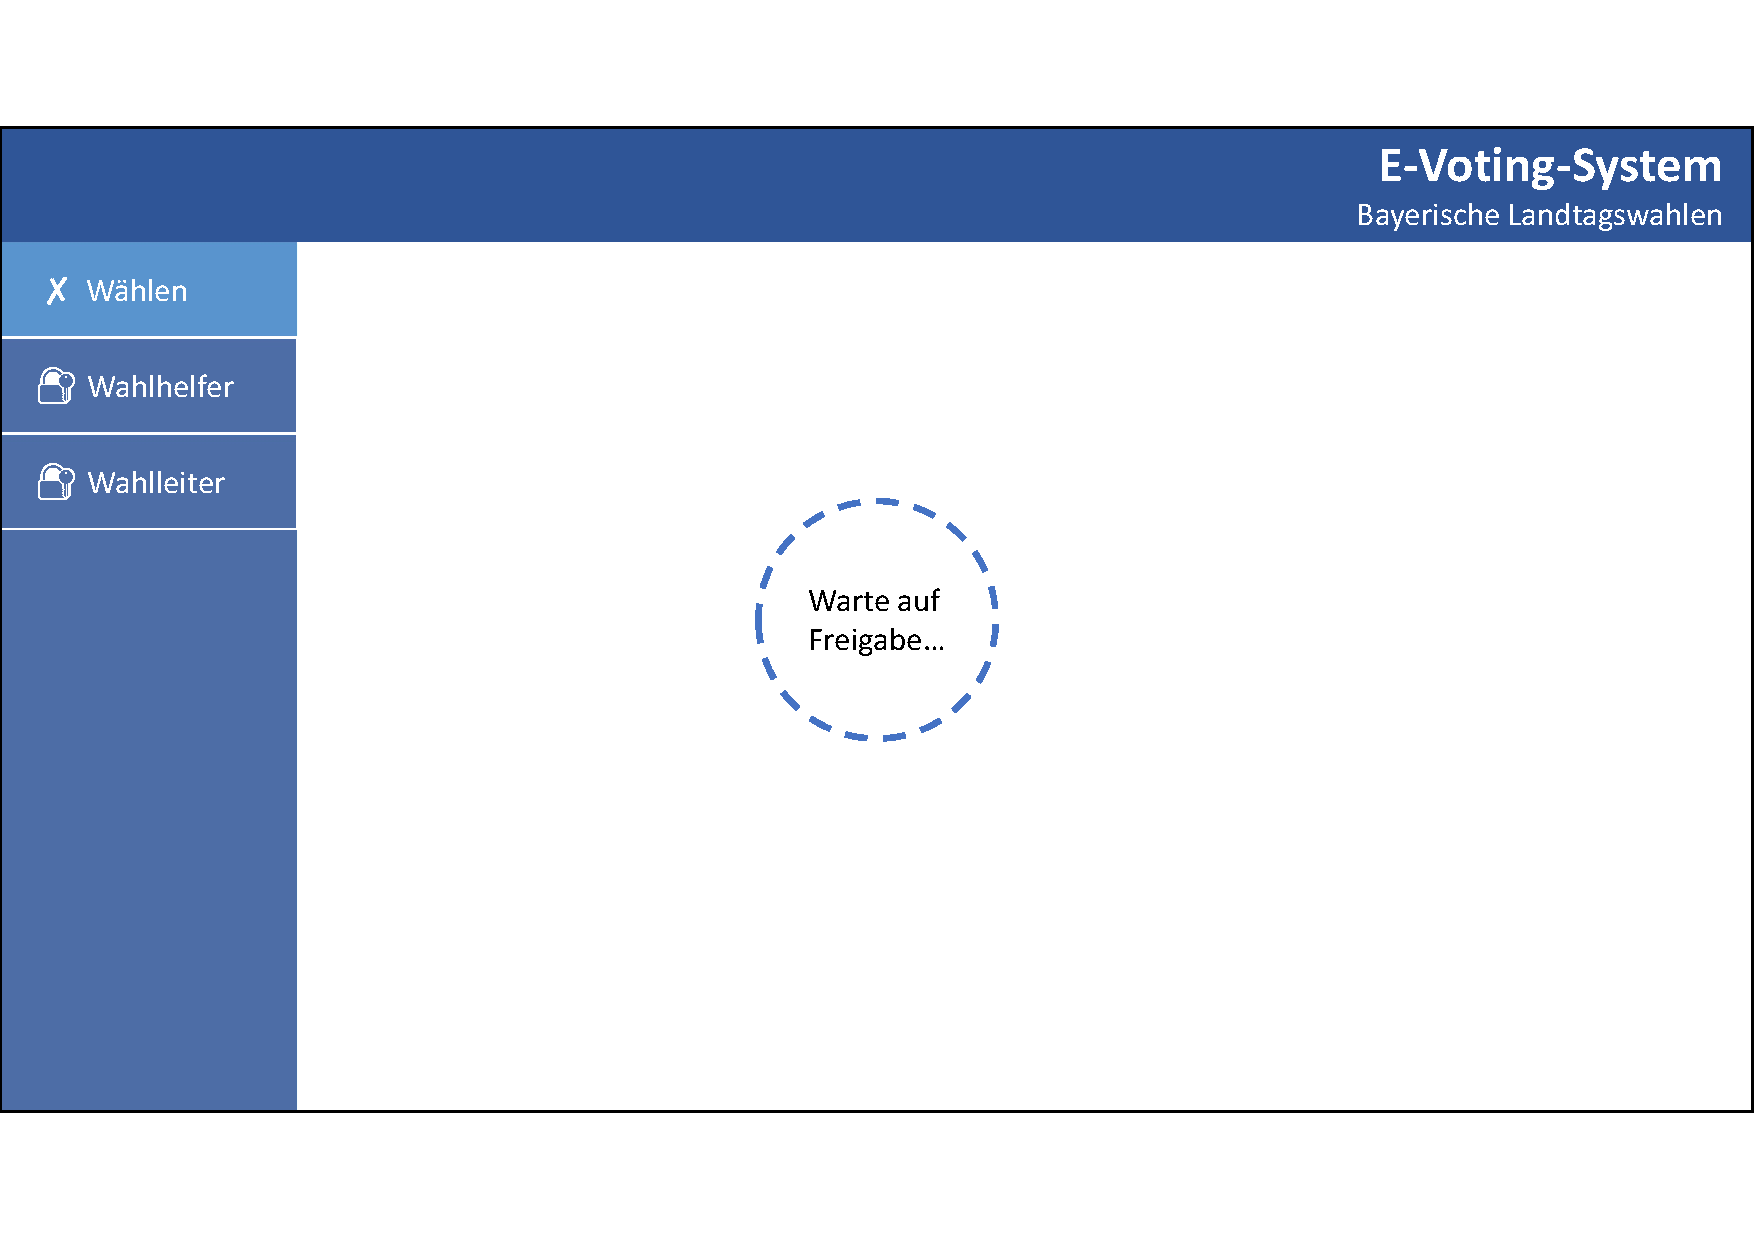
\includepdf[nup=1x2, pages=-,templatesize={\textwidth}{10cm}]{../Mock.pdf}

\section{Datenmodell}
Das Datenmodell ergibt sich aus den Anforderungen und dem Vorschlag des Lastenhefts wie folgt:
\begin{itemize}
  \item \textbf{Wahl} - Repräsentation einer einzelnen Wahl an einem festen Datum. 
        Durch letzteres Merkmal ist es möglich mehrere Wahlen in einem Jahr festzuhalten.
  \item \textbf{Stimme} - Jede(r) WählerIn besitzt je eine Erst- und Zweitstimme, welche er oder sie in ihrem
        Stimmbezirk für KandidatInnen oder eine Partei abgeben können. Mit der Erststimme wählt eine wahlberechtigte Person
        primär den oder die von ihr bevorzugten DirektkandidatIn ihres Stimmkreises. Über die Zweitstimme wählt 
        jede wahlberechtigte Person genau einen Kandidaten einer Liste aus ihrem Regierungsbezirk oder eine Partei, bzw. deren Liste. 
        Das prozentuale Gesamtabschneiden einer Partei aus kombinierten Erst- und Zweitstimmen ist für das 
        Wahlergebnis relevant.
  \item \textbf{Regierungsbezirk} - Bayern ist in sieben Regierungsbezirke unterteilt: Oberbayern,
        Niederbayern, Schwaben, Ober-, Unter-, Mittelfranken und Oberpfalz. Jeder Regierungsbezirk
        hat eine unterschiedliche Anzahl zu vergebender Direkt- und Listenmandate.
  \item \textbf{Stimmkreis} - Regierungsbezirke sind gemäß Bevölkerungszahlen in Stimmkreise aufgeteilt.
        Pro Stimmkreis wird ein(e) DirektkandidatIn gewählt.
  \item \textbf{RBInfo}/\textbf{SKInfo} - Zusatzinformationen zum Regierungsbezirk bzw. Stimmkreis,
        welche sich pro Wahl ändern können, werden hier gespeichert.
  \item \textbf{KandidatIn} - Eine sich zur Wahl stellende Person mit notwendigen persönlichen Angaben. 
        Insbesondere kann ein(e) KandidatIn als DirektkandidatIn für einen Stimmkreis aufgestellt sein.
  \item \textbf{Partei} - KandidatInnen sind Mitglied einer Partei und können sich von dieser für einen 
        Listenplatz aufstellen lassen
  \item \textbf{Liste} - Jede Partei kann pro Regierungsbezirk eine Liste mit KandidatInnen, welche Mitglieder der 
        Partei sind, aufstellen. Listenplätze ändern sich durch die Anzahl erhaltener Stimmen. Listenmandate
        einer Partei werden dann nach finaler Listenreihenfolge berechnet.
  \item \textbf{Wahlhelfer} - Wahlhelfer überwachen und authentifizieren Wahlkabinen und Wähler
  \item \textbf{Wahlkabine} - Wähler geben ihre Stimmen in Wahlkabinen ab
\end{itemize}

\begin{center}
	\includegraphics[page=2,width=\textwidth]{../model.pdf}
\end{center}

\section{Globale Testfälle und Szenarien}
\begin{center}
      \begin{tabular}{|m{3.5cm}|m{12cm}|}
        \hline
        \rowcolor{TUMBlue} \textcolor{white}{\textbf{Szenario}} & \textcolor{white}{\textbf{Abnahmekriterium}} \\
        \hline
        Stimmabgabe & 10~ Stimmabgaben können pro Sekunde erfolgen \\
        \hline
        Auswertung & Es muss möglich sein 100 Analyseanfragen pro Sekunde zu bearbeiten \\
        \hline
      \end{tabular}
\end{center}

\clearpage
%%%%%%%%%%%%%%%%%%%%%%%%%%%%%%%%%%%%%%%%%%%%%%%%%%%%%%%%%%%%%%%%%%%%%%
% Begriffslexikon zur Beschreibung des Produkts						 %
%%%%%%%%%%%%%%%%%%%%%%%%%%%%%%%%%%%%%%%%%%%%%%%%%%%%%%%%%%%%%%%%%%%%%%
%\newglossaryentry{sortierschluessel}
%{
%  name=Sortierschlüssel,
%  description={ein Schlüssel, anhand dessen diese Einträge sortiert werden}
%}
\newglossaryentry{Technologiestack}
{
  name=Technologiestack,
  description={Sammlung aller verwendeten Technologien im Projekt. Gegebenenfalls hierarchisch sortiert wenn aufeinander aufbauend}
}
\newglossaryentry{Client}
{
  name=Client,
  description={Programm, dass die Dienste eines Servers in Anspruch nimmt}
}
\newglossaryentry{Server}
{
  name=Server,
  description={Rechner, der für andere in einem Netzwerk mit ihm verbundene Systeme bestimmte Aufgaben übernimmt und von dem diese ganz oder teilweise abhängig sind}
}
\newglossaryentry{Datenbanksystem}
{
  name=Datenbanksystem,
  description={Ein Datenbanksystem (DBS) ist eine systematisch strukturierte, langfristig verfügbare Sammlung von Daten einschließlich der zur Verwaltung notwendigen Software}
}
\newglossaryentry{OLAP}
{
  name=OLAP,
  description={Online Analytical Processing}
}
\newglossaryentry{OLTP}
{
  name=OLTP,
  description={Online Transaction Processing}
}


% Setze den richtigen Namen für das Glossar
\renewcommand*{\glossaryname}{\section{\glossarName}}

% Drucke das gesamte Glossar
\glsaddall
\printglossaries

% Trage das Glossar in das Inhaltsverzeichnis ein
\stepcounter{section}
\addcontentsline{toc}{section}{\numberline {\thesection} \glossarName}
\end{document}
